% Created 2025-01-14 Tue 22:47
% Intended LaTeX compiler: pdflatex
\documentclass[presentation]{beamer}
\usepackage[utf8]{inputenc}
\usepackage[T1]{fontenc}
\usepackage{graphicx}
\usepackage{amsmath, amssymb}
\usepackage{hyperref}
\setbeamertemplate{navigation symbols}{}
\usepackage[utf8]{inputenc}
\usepackage[T1]{fontenc}
\usepackage{graphicx}
\usepackage{longtable}
\usepackage{wrapfig}
\usepackage{rotating}
\usepackage[normalem]{ulem}
\usepackage{amsmath}
\usepackage{amssymb}
\usepackage{capt-of}
\usepackage{hyperref}
\nocite{*}
\usepackage[T1]{fontenc}
\usepackage[utf8]{inputenc}
\usepackage[spanish]{babel}
\usepackage[backend=biber, style=apa]{biblatex}
\addbibresource{/home/iccd332-josune/expo/ExposicionArqui/bibliography.bib}
\author{Martín Cusme, Celeste Gallardo, Josune Singaña, Richard Tipantiza}
\date{}
\title{S9-Memoria-del-Sistema}
\hypersetup{
 pdfauthor={Martín Cusme, Celeste Gallardo, Josune Singaña, Richard Tipantiza},
 pdftitle={S9-Memoria-del-Sistema},
 pdfkeywords={},
 pdfsubject={},
 pdfcreator={Emacs 27.1 (Org mode 9.3)}, 
 pdflang={Spanish}}
\begin{document}

\maketitle
\tableofcontents



\section{Indicaciones}
\label{sec:org01efdb0}
\subsection{Indicaciones}
\label{sec:org8cd161b}


\section{Sobre este Documento}
\label{sec:org7512190}
\subsection{Sobre este Documento}
\label{sec:orga9e434c}
\begin{itemize}
\item Este documento tiene la propuesta de temas a tratar y desarrollar por los estudiantes.
\item Se ha de utilizar como base la bibliografía recomendada, pero puede consultar bibliografía adicional.
\end{itemize}


\section{Memoria Cache (E2, 11, 162)}
\label{sec:orga7af681}
\subsection{Principios Básicos de las Memorias Caché (E2,11,163)(E2,7,133)}
\label{sec:org781b4ea}
\begin{enumerate}
\item ¿Para que sirve?
\label{sec:org19be1e6}
\begin{itemize}
\item El objetivo principal de la memoria caché es mejorar la velocidad de acceso a los datos almacenados, combinando el acceso rápido a datos de una memoria más cara y de alta velocidad (memoria caché) con el almacenamiento más lento pero de mayor capacidad de la memoria principal.
\end{itemize}

\item Funcionamiento
\label{sec:orgb00648f}
\begin{itemize}
\item La CPU transfiere palabras o bloques entre la caché y la memoria principal. La caché actúa como intermediaria rápida entre la CPU y la memoria principal, almacenando temporalmente datos que la CPU necesita frecuentemente.
\end{itemize}
\end{enumerate}

\subsection{Principios Básicos de las Memorias Caché (E2,11,163)(E2,7,133)}
\label{sec:org85b7ace}

\begin{itemize}
\item En el modelo simple de caché (como muestra la Figura 5.1a), la CPU realiza transferencias rápidas a la caché y transferencias más lentas a la memoria principal.
\end{itemize}

\begin{center}
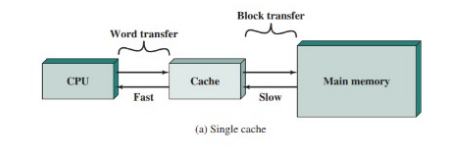
\includegraphics[width=.9\linewidth]{./Imagenes/captura1.png}
\end{center}


\subsection{Principios Básicos de las Memorias Caché (E2,11,163)(E2,7,133)}
\label{sec:orga82a7e4}

\subsection{Niveles de Caché:}
\label{sec:org9a0a093}
\begin{itemize}
\item Se organizan en varios niveles (L1, L2, L3). A medida que se avanza en los niveles, la velocidad disminuye, pero la capacidad aumenta.
\begin{itemize}
\item Caché de Nivel 1 (L1): La más rápida y de menor capacidad.
\item Caché de Nivel 2 (L2): Un poco más lenta, pero con mayor capacidad.
\item Caché de Nivel 3 (L3): Menos rápida que L1 y L2, pero aún más rápida que la memoria principal.
\end{itemize}
\end{itemize}


\subsection{Elementos de Diseño de la memoria Caché}
\label{sec:org0a30f60}

\subsection{Introducción a la Caché}
\label{sec:orgf497d53}
\begin{itemize}
\item "La memoria caché mejora la velocidad de acceso al reducir la distancia entre el procesador y la memoria principal."
\item "Los fallos de caché generan tráfico en el bus del sistema."
\end{itemize}

\begin{center}
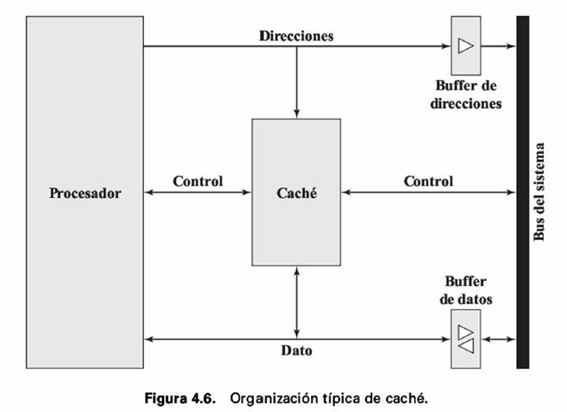
\includegraphics[width=.9\linewidth]{./Imagenes/fig4.6.png}
\end{center}


\subsection{Parámetros de Diseño de la Caché}
\label{sec:org325a38a}
\begin{enumerate}
\item Parámetros Principales
\label{sec:org4ad0d8c}
\begin{itemize}
\item "La función de correspondencia, el tamaño de línea y el algoritmo de sustitución son clave para el diseño de una caché eficiente."
\item "La jerarquía de cachés puede mejorar el rendimiento en aplicaciones bien optimizadas."
\end{itemize}

\begin{center}
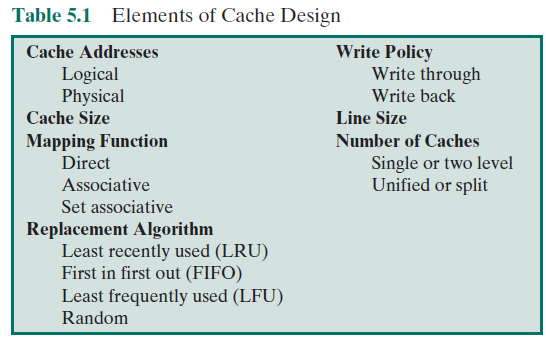
\includegraphics[width=.9\linewidth]{./Imagenes/tabla5.1.png}
\end{center}
\end{enumerate}


\subsection{Tamaño Caché}
\label{sec:org8bd8887}
\begin{enumerate}
\item Consideraciones de Tamaño
\label{sec:orgbc85849}
\begin{itemize}
\item "El tamaño de la caché impacta directamente en su velocidad y costo."
\item "No existe un tamaño 'óptimo' único, ya que depende de la naturaleza de las tareas."
\end{itemize}

\begin{center}
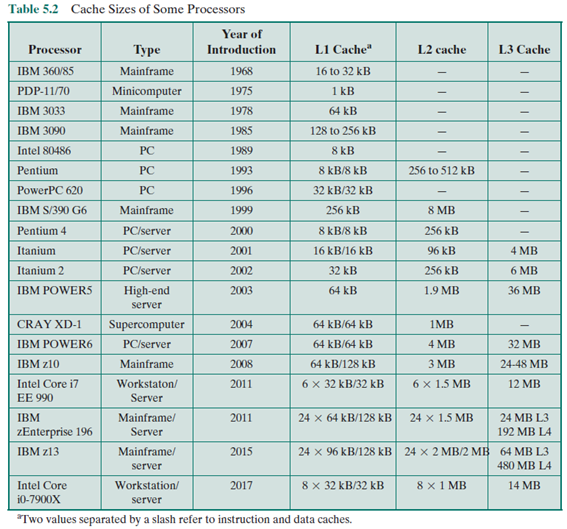
\includegraphics[width=.9\linewidth]{./Imagenes/tabla5.2.png}
\end{center}
\end{enumerate}

\subsection{Tipos de caché}
\label{sec:org7068f7d}
\begin{enumerate}
\item Clasificación
\label{sec:org4ccf07e}
\begin{itemize}
\item "La caché lógica utiliza direcciones virtuales; la física, direcciones físicas."
\item "La caché lógica puede ser más rápida pero requiere mayor gestión en cambios de contexto."
\end{itemize}

\begin{center}
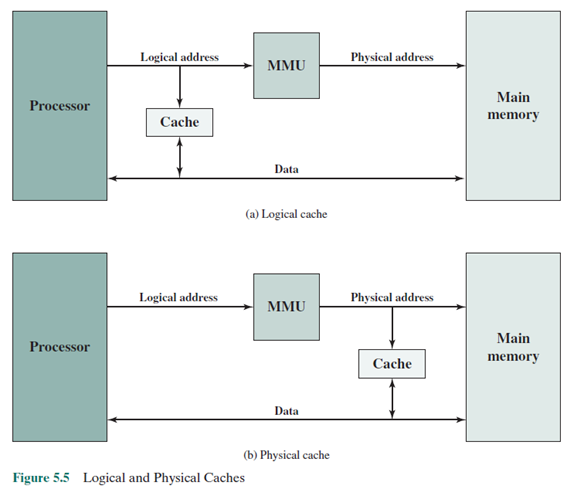
\includegraphics[width=.9\linewidth]{./Imagenes/fig5.png}
\end{center}
\end{enumerate}




\subsection{Función de Correspondencia (E2,11,170)(E2,7,137)}
\label{sec:orge51c53c}
\begin{enumerate}
\item Técnicas de Organización
\label{sec:org8de9f13}
Se requiere un algoritmo que permita asociar los bloques de memoria principal con las líneas de caché, ya que hay menos líneas de caché que bloques de memoria. Además, es necesario un método para identificar qué bloque de memoria está ocupando una línea específica. Para organizar la caché, se utilizan tres técnicas principales: correspondencia directa, asociativa y asociativa por conjuntos, las cuales serán explicadas junto con ejemplos concretos.
El texto explica tres técnicas para organizar la caché:

\begin{itemize}
\item \textbf{\textbf{Correspondencia directa:}} Cada bloque de memoria principal se asigna a una línea de caché específica. Por ejemplo, el bloque 10 se asigna a la línea 10 mod 8 = 2.

\item \textbf{\textbf{Correspondencia asociativa:}} Cualquier bloque puede ocupar cualquier línea de caché, lo que ofrece más flexibilidad, pero es más lento de buscar.

\item \textbf{\textbf{Correspondencia asociativa por conjuntos:}} La caché se divide en conjuntos, y cada bloque puede ocupar cualquier línea dentro de un conjunto específico. Por ejemplo, el bloque 10 se asigna al conjunto 10 mod 4 = 2.
\end{itemize}

Estas técnicas optimizan la asignación de memoria y el uso eficiente de la caché.
\end{enumerate}

\section{Algoritmo de Sustitución}
\label{sec:org655ddab}
\subsection{Algoritmo de Sustitución (E2,7,148)}
\label{sec:org3721374}
\begin{enumerate}
\item Tipos de Algoritmos
\label{sec:org2667070}
Una vez llena la caché, se debe reemplazar un bloque existente para introducir uno nuevo.
En correspondencia directa, no hay elección, ya que cada bloque tiene una línea específica.
En técnicas asociativas, se requieren algoritmos de sustitución implementados en hardware para alta velocidad.\autocite{stallings2006organización}
\begin{enumerate}
\item LRU (Least Recently Used)
\item FIFO (First-In-First-Out
\item LFU (Least Frequently Used
\item Aleatoria
\end{enumerate}
\end{enumerate}

\section{Política de escritura}
\label{sec:org750b167}
\subsection{Política de escritura}
\label{sec:orgb5fdbe9}
\begin{itemize}
\item Casos de reemplazo en caché
\begin{enumerate}
\item Casos de reemplazo en caché
\item Casos de reemplazo en caché
\end{enumerate}
\item Problemas al reemplazar bloques
\begin{enumerate}
\item Acceso múltiple a la memoria principal
\item Sistemas multiprocesado
\end{enumerate}
\item Sistemas multiprocesado
\begin{enumerate}
\item Escritura inmediata
\item Postescritura
\end{enumerate}
\item Estadísticas de escritura
\item Vigilancia del bus con escritura inmediata
\item Transparencia hardware
\item Memoria excluida de caché
\end{itemize}

\section{Tamaño de Linea}
\label{sec:orgfe2b2c6}
\subsection{Tamaño de Línea}
\label{sec:orgbc0a72e}
\begin{itemize}
\item Tamaño de línea de caché:
\item Efectos al aumentar el tamaño del bloque:
\begin{enumerate}
\item Reducción de bloques en caché
\item Mayor distancia de las palabras adicionales:
\end{enumerate}
\item Relación compleja entre tamaño y tasa de aciertos
\end{itemize}
\subsection{Número de Cachés (E2, 7, 150)}
\label{sec:orgff3abd1}
Inicialmente, los sistemas contaban con una sola caché, pero con el tiempo se ha vuelto común utilizar múltiples cachés. Este diseño incluye consideraciones como el número de niveles de caché y el uso de cachés unificadas o separadas. Las cachés separadas evitan la competencia entre instrucciones y datos, mejorando el rendimiento en sistemas avanzados.

\textbf{\textbf{Cachés Multinivel}}
Las cachés on-chip, integradas en el procesador, reducen el uso del bus externo y mejoran el rendimiento. Normalmente, se complementan con una caché externa (L2). Los diseños más recientes incluyen múltiples niveles: L1, L2 y, en algunos casos, L3. Estas cachés adicionales, ahora frecuentemente on-chip, mejoran significativamente el rendimiento al reducir los tiempos de acceso a memoria, aunque complican aspectos como tamaño, políticas de escritura y algoritmos de reemplazo.

\textbf{\textbf{Caché Unificada}}
Las cachés unificadas almacenan tanto instrucciones como datos en un único espacio, maximizando la tasa de aciertos al adaptarse dinámicamente a las necesidades de ejecución. Además, solo requieren un diseño único, simplificando la implementación.

\textbf{\textbf{Cachés Separadas}}
Por otro lado, las cachés separadas para instrucciones y datos son preferidas en sistemas super-escalares y con segmentación de cauce. Este diseño elimina la competencia por recursos entre la ejecución de instrucciones y la unidad de datos, mejorando el rendimiento y optimizando la ejecución paralela de instrucciones.

\section{Referencias}
\label{sec:org51a2802}
\subsection{Bibliografía}
\label{sec:orgcbb9b91}
\printbibliography
\end{document}
